%%% Hlavní soubor. Zde se definují základní parametry a odkazuje se na ostatní části. %%%

%% Verze pro jednostranný tisk:
% Okraje: levý 40mm, pravý 25mm, horní a dolní 25mm
% (ale pozor, LaTeX si sám přidává 1in)
\documentclass[12pt,a4paper]{report}
\setlength\textwidth{145mm}
\setlength\textheight{247mm}
\setlength\oddsidemargin{15mm}
\setlength\evensidemargin{15mm}
\setlength\topmargin{0mm}
\setlength\headsep{0mm}
\setlength\headheight{0mm}
% \openright zařídí, aby následující text začínal na pravé straně knihy
\let\openright=\clearpage

%% Pokud tiskneme oboustranně:
% \documentclass[12pt,a4paper,twoside,openright]{report}
% \setlength\textwidth{145mm}
% \setlength\textheight{247mm}
% \setlength\oddsidemargin{15mm}
% \setlength\evensidemargin{0mm}
% \setlength\topmargin{0mm}
% \setlength\headsep{0mm}
% \setlength\headheight{0mm}
% \let\openright=\cleardoublepage

%% Pokud používáte csLaTeX (doporučeno):
\usepackage{czech}
%% Pokud nikoliv:
%\usepackage[czech]{babel}
%\usepackage[T1]{fontenc}

%% Použité kódování znaků: obvykle latin2, cp1250 nebo utf8:
%\usepackage[latin2]{inputenc}
\usepackage[utf8]{inputenc}

%% Ostatní balíčky
\usepackage{graphicx}
\usepackage{amsthm}
%\usepackage[pdftex]{graphicx}

\usepackage{url}
\DeclareUrlCommand\url{\def\UrlLeft{<}\def\UrlRight{>} \urlstyle{tt}}

%% Balíček hyperref, kterým jdou vyrábět klikací odkazy v PDF,
%% ale hlavně ho používáme k uložení metadat do PDF (včetně obsahu).
%% POZOR, nezapomeňte vyplnit jméno práce a autora.
\usepackage[ps2pdf,unicode]{hyperref}   % Musí být za všemi ostatními balíčky
\hypersetup{pdftitle=AJAX CAT --- webový editor s podporou pro překlad}
\hypersetup{pdfauthor=Ondřej Odcházel}

%%% Drobné úpravy stylu

% Tato makra přesvědčují mírně ošklivým trikem LaTeX, aby hlavičky kapitol
% sázel příčetněji a nevynechával nad nimi spoustu místa. Směle ignorujte.
\makeatletter
\def\@makechapterhead#1{
  {\parindent \z@ \raggedright \normalfont
   \Huge\bfseries \thechapter. #1
   \par\nobreak
   \vskip 20\p@
}}
\def\@makeschapterhead#1{
  {\parindent \z@ \raggedright \normalfont
   \Huge\bfseries #1
   \par\nobreak
   \vskip 20\p@
}}
\makeatother

% Toto makro definuje kapitolu, která není očíslovaná, ale je uvedena v obsahu.
\def\chapwithtoc#1{
\chapter*{#1}
\addcontentsline{toc}{chapter}{#1}
}




\def\samp#1{{\textit{#1}}} % ukazkovy text
\def\url#1{{\texttt{#1}}}
\def\footurl#1{\footnote{\url{#1}}}
\def\equo#1{{``{#1}''}}

\def\parcite#1{\cite{#1}}  % should look like e.g. (Bojar, 2009)
\def\perscite#1{\cite{#1}}  % should look like e.g. Bojar (2009)

\def\Fref#1{Figure~\ref{#1}}
\def\Sref#1{Section~\ref{#1}}




\begin{document}

% Trochu volnější nastavení dělení slov, než je default.
\lefthyphenmin=2
\righthyphenmin=2

%%% Titulní strana práce

\pagestyle{empty}
\begin{center}

\large

Univerzita Karlova v Praze

\medskip

Matematicko-fyzikální fakulta

\vfill

{\bf\Large BAKALÁŘSKÁ PRÁCE}

\vfill

\centerline{\mbox{\includegraphics[width=60mm]{logo.eps}}}

\vfill
\vspace{5mm}

{\LARGE Ondřej Odcházel}

\vspace{15mm}

% Název práce přesně podle zadání
{\LARGE\bfseries AJAX CAT --- webový editor s podporou pro překlad}

\vfill

% Název katedry nebo ústavu, kde byla práce oficiálně zadána
% (dle Organizační struktury MFF UK)
Ústav formální a aplikované lingvistiky

\vfill

\begin{tabular}{rl}

Vedoucí bakalářské práce: & RNDr. Ondřej Bojar, Ph.D. \\
\noalign{\vspace{2mm}}
Studijní program: & Informatika \\
\noalign{\vspace{2mm}}
Studijní obor: & Programování \\
\end{tabular}

\vfill

% Zde doplňte rok
Praha 2011

\end{center}

\newpage

%%% Následuje vevázaný list -- kopie podepsaného "Zadání diplomové práce".
%%% Toto zadání NENÍ součástí elektronické verze práce, nescanovat.

%%% Na tomto místě mohou být napsána případná poděkování (vedoucímu práce,
%%% konzultantovi, tomu, kdo zapůjčil software, literaturu apod.)

\openright

\noindent
Poděkování.

\newpage

%%% Strana s čestným prohlášením k diplomové práci

\vglue 0pt plus 1fill

\noindent
Prohlašuji, že jsem tuto diplomovou práci vypracoval samostatně a výhradně
s~použitím citovaných pramenů, literatury a dalších odborných zdrojů.

\medskip\noindent
Beru na~vědomí, že se na moji práci vztahují práva a povinnosti vyplývající
ze zákona č. 121/2000 Sb., autorského zákona v~platném znění, zejména skutečnost,
že Univerzita Karlova v Praze má právo na~uzavření licenční smlouvy o~užití této
práce jako školního díla podle §60 odst. 1 autorského zákona.

\vspace{10mm}

\hbox{\hbox to 0.5\hsize{%
V Praze dne 27. května 2011
\hss}\hbox to 0.5\hsize{%
Podpis autora
\hss}}

\vspace{20mm}
\newpage

%%% Povinná informační strana diplomové práce

\vbox to 0.5\vsize{
\setlength\parindent{0mm}
\setlength\parskip{5mm}

Název práce:
AJAX CAT --- webový editor s podporou pro překlad
% přesně dle zadání

Autor:
Ondřej Odcházel

Katedra:  % Případně Ústav:
Ústav formální a aplikované lingvistiky
% dle Organizační struktury MFF UK

Vedoucí bakalářské práce:
RNDr. Ondřej Bojar, Ph.D., Ústav formální a aplikované lingvistiky
% dle Organizační struktury MFF UK, případně plný název pracoviště mimo MFF UK

Abstrakt:
% abstrakt v rozsahu 80-200 slov; nejedná se však o opis zadání diplomové práce
Cílem této práce je implementace systému pro podporu překladu. Systém je rozdělen na serverovou a klientskou část. Serverová část využívá systém strojového překladu ke generování nápověd při překladu. Prvním druhem nápovědy je tabulka s různými variantami překladu každé fráze překládaného textu. Dalším druhem nápovědy jsou návrhy překladu. Tyto návrhy v každé fázi překladu představují nejpravděpodobnější možnosti pokračování překladu. Klientská část systému je webová aplikace ovládaná překladatelem, kterému nabízí nápovědy získané ze serveru. Kromě toho se také klientská část stará o jednoduchou správu překladových dokumentů.

Klíčová slova:
% 3 až 5 klíčových slov
překlad, webová aplikace, CAT

\vss}\nobreak\vbox to 0.49\vsize{
\setlength\parindent{0mm}
\setlength\parskip{5mm}

Title:
% přesný překlad názvu práce v angličtině
AJAX CAT --- web editor with support for translation

Author:
Ondřej Odcházel

Department:
Institute of Formal and Applied Linguistics
% dle Organizační struktury MFF UK v angličtině

Supervisor:
RNDr. Ondřej Bojar, Ph.D., Institute of Formal and Applied Linguistics
% dle Organizační struktury MFF UK, případně plný název pracoviště
% mimo MFF UK v angličtině

Abstract:
% abstrakt v rozsahu 80-200 slov v angličtině; nejedná se však o překlad
% zadání diplomové práce

Keywords:
% 3 až 5 klíčových slov v angličtině
translation, web application, CAT

\vss}

\newpage

%%% Strana s automaticky generovaným obsahem diplomové práce. U matematických
%%% prací je přípustné, aby seznam tabulek a zkratek, existují-li, byl umístěn
%%% na začátku práce, místo na jejím konci.

\openright
\pagestyle{plain}
\setcounter{page}{1}
\tableofcontents

%%% Jednotlivé kapitoly práce jsou pro přehlednost uloženy v samostatných souborech
%\chapter*{Úvod}
\addcontentsline{toc}{chapter}{Úvod}

Díky novým statistickým přístupům zažívá obor strojového překladu jazyka v posledních letech opět velký rozvoj. Nové výpočetní i algoritmické možnosti umožňují vytváření stále lepších jazykových překladů. Stále se však nepodařilo vytvořit univerzální překladový systém, který by dokázal nahradit lidské překladatele, ani v jednom běžném jazykovém páru. Je stále otázka zdali se podobný překladový systém v budoucnosti lidstvu podaří sestavit. Již dnes jsou ale překladové systémy na úrovni, která sice nedokáže překladatele nahradit, ale v mnoha odvětvích usnadňuje jejich práci. Překladové systémy již nyní poskytují alespoň nápovědu, jak daný text přeložit. Překladatel však stále musí výstup z takového systému kontrolovat a editovat. Každý z těchto editačních zásahů představuje pro překladatele komplikaci a pokud je množství nutných zásahů nad nějakou hranicí, překladatel raději místo editování výstupu překladového systému vytvoří překlad sám. Pro zjednodušení překladatelské práce je tedy potřeba nejen zlepšovat tyto překladové systémy, ale také software kteří překladatelé pro interakci s překladovým systémem používají. Překladový software, který využívá pro nápovědu překladatelům strojový překlad je speciální případem CAT (computer--aided translation) systému.

Cílem této bakalářské práce je implementace jednoho CAT systému. Pro podporu překladu bude systém využívat překladový systém Moses. Celý projekt je rozdělen do dvou částí --- serverová a klientská část. Implementací serverové části bude vytvořen HTTP server. Tento server bude spouštět Mosese a skrz HTTP požadavky bude poskytovat klientovi odpovědi. Požadavky budou dvojího typu. Klient se může systému zeptat na překlad věty v určité jazyce. Server pak odpoví tabulkou překladových možností. Sloupce této tabulky jsou jednotlivé úseky ve zdrojovém překladovém úseku (typicky slova ve větě). V řádcích tabulky jsou pak přeložené úseky textu v cílovém jazyce. Úseky jsou seřazeny v tabulce tak, že čím výše je daný úsek, tím větší je pravděpodobnost toho, že se jedná o "správný překlad". Taková to tabulka je jedním ze základů implementovaného CAT systému.

Dalším typem klientského požadavku bude jakási lokální nápověda během překladu. Jedná se o podobný druh nápovědy jakou nám poskytují například intenetové vyhledávače. V nich často uživatel nemusí psát celý vyhledávací dotaz a může využí nápovědy, která mu nabízí nejběžnější podobné dotazy. Podobně i implementovaný server bude dávat nápovědu, jak dále pokračovat s překladem. Aby překladový systém mohl tuto nápovědu poskytnout, pořebuje znát tři parametry. Text ve zdrojovém jazyce, vektor určující, které úseky jsou již přeloženy a již přeložená část věty v cílovém jazyce. Cílem této práce je i rozšířit možnosti Mosese tak, aby s těmito třemi parametry dokázal pracovat a vygeneroval nápovědu, jak v překladu pokračovat.

Samotná serverová část tak bude moci fungovat jako komponenta samostatně a poskytovat nápovědu k překladu i jiném CAT systému.

Druhou částí práce je implementace klientské části CAT systému. Tato část bude sloužit k interakci překladatele s překladový systémem. Tato interakce by měla být co nejvíce přátelská k uživateli. Ten typicky zadá zdrojový text pro překlad a zdrojový a cílový jazyk překladu. CAT systém tento zdrojový text rozseká do bloků (typicky vět) a ke každé větě překladateli nabídne nápovědu generovanou v serverové části. Součástí implementace klientské části bude i jednoduchý systém pro zprávu obsahu, aby překladatel mohl pokračovat v překladu i po znovuotevření aplikace. Klientská část bude podobně jako serverová část fungovat sama o sobě. Pokud tedy nebude napojena na server, může pracovat sama o sobě jako systém pro správu překladů.



%
\chapter{Překlad a strojový překlad}

\section{Překladové problémy}

Překlad je proces přenesení významu z textu ve zdrojovém jazyce do jazyka cílového. Úloha překladu je složitá i tím, že žádný výsledek nejde označit za nejlepší. Že neexistuje dokonalý překlad lze ilustrovat na překladech knih, nebo divadelních her. Hry Williama Shakespearea byly z angličtiny do češtiny přeloženy mnohokrát, přesto jsou stále inscenovány hry s různými překlady.

Bez hlubších jazykových znalostí se může jevit úloha překladu snadná, mezi většinou jazyků máme přeci slovník. Ale pokud chceme přeložit anglické slovo "house" do češtiny, můžeme mít problém. Ve většině případů lze toto slovo přeložit jako "dům". Pokud ale překládáme text o anglické královně, kde se objeví sousloví "House of Windsor", zřejmě není řeč o domu, kde bydlí Windsorové, ale o "rodu Windsorů". Překladatel tedy při textu potřebuje znát kontext ve kterém je slovo použito a často také potřebuje mít odborné znalosti z oboru překládaného textu.

Jazyk není neměnný a v průběhu času se vyvíjí. Můžeme to vidět například na Bibli. Její nejznámější překlad, Bible Kralická je přes 300 (?) let starý. Vznikají proto nové překlady, které jsou dnešním čtenářům přístupnější. Žádný překlad tedy nelze označit za dokonalý a navždy správný.

\section{Historie strojového překladu}

Na počátku dějin strojového překladu stála, podobně jako v mnoha jiných oborech, armáda. Spojené státy Americké byli v padesátých letech ve Studené válce se Sovětským svazem. V této válce beze zbraní sehráli velkou úlohu i výzvědné služby, které zachytávali velké množství nepřátelských zpráv. Tyto zprávy bylo nutné co nejrychleji přeložit. A právě v této době se zrodila myšlenka použít k tomuto účelu počítače, které byli produktem předchozího válečného konfliktu, 2. světové války. ( http://www.hutchinsweb.me.uk/GU-IBM-2005.pdf ) Významnou demonstrací použití strojového překladu se v roce 1954 stal takzvaný Georgetownský experiment. Pro tento experiment vyvinula Georgetownská univerzita spolu s firmou IBM překladový systém pro překlad z ruštiny do angličtiny. Tento systém používal slovník 250 slov a 6 gramatických pravidel. Jeho doménou byly zejména překlady v oblasti chemie. Během experimentu bylo přeloženo více než 60 vět. Experiment byl všeobecně přijat jako úspěch, což donutilo americkou vládu investovat v následujících letech do oblasti strojového překladu.

Následovaly léta práce zejména v SSSR a USA na systémech pro automatické překlady zejména mezi ruštinou a angličtinou. Žádný dobře použitelný systém, který by poskytoval uspokojivé výsledky, však nevzniknul. Pochybnosti ohledně možností strojového překladu vyjádřil na konci padesátých let lingvista Yehoshua Bar-Hillel. Ten argumentoval pomocí anglické věty "The box was in the pen." Překlad této věty by mohl být: "Pero bylo v ohradě." Jelikož anglické slovo "pen" znamená "pero" i "ohrada", musí mít překladový systém, který chce větu přeložit správně, sémantickou informaci, která by mu napověděla, že krabice nemůže být peru, tedy že správným překladem slova "pen" do češtiny je v tomto kontextu slovo "ohrada".

http://www.hutchinsweb.me.uk/ALPAC-1996.pdf
I z tohoto důvodu bylo vytvoření komplexního překladového systému v té době zřejmě nemožné. Americká vláda však dále pokračuje ve financování výzkumu. V roce 1966 vyšla zpráva skupiny ALPAC (Automatic Language Processing Advisory Committee). Která doporučovala americké vládě další postup při financování překladového výzkumu. Zpráva zmenšovala optimismus, vyvolaný zejména Georgetownským experimentem, že se v dohledné době podaří vytvořit kvalitní systém pro strojový překlad. Výsledkem bylo téměř úplné zastavení financování výzkumu americkou vládou. Výzkum dále pokračoval zejména v Evropě, nebo Kanadě. Právě v kanadském Montrealu vznikl systém METEO. Ten byl v letech 1981 až 2001 používán pro překlad meteorologických zpráv mezi angličtinou a francouzštinou. Právě omezená překladová doména systému umožnila nabízet kvalitní překlady předpovědí počasí.


\section{Součastnost strojového překladu}
V posledních letech spolu s pokračující globalizací světa a stále vyšší penetrací internetového připojení se zvyšuje i poptávka po překladech. Nadnárodní firmy potřebují při svém růstu stále více překladů. Dalším impulzem zvyšujícím popávku po překladech je i rozšiřování Evropské Unie. V součastnosti unie používá 23 oficiálních jazyků ve kterých musí být přístupné všechny důležité úřední dokumenty. Tvorba tolika překladů je velice pracná a nákladná, což vytváří poptávku po zjednodušením procesu překladu.

Výpočetní výkon počítačů stále roste rychlostí Mooreova zákona (ftp://download.intel.com/research/silicon/moorespaper.pdf), což v posledních letech otevřelo možnosti pro použití statistických metod ve strojovém překladu. Toho využívá statistický překladový systém Moses, open-source překladový systém, který používám i ve svém projektu a cílem projektu byla i implementace nových rozšíření. Dalším známým statistickým překladovým systémem je Google Translate.

Kromě systému využívajících statických postupů se stále vyvíjí i pravidlové překladové systémy. Kromě mnoha proprietálních systémů bych zmínil open-source systém Apertium. Stejně jako u dalších podobných systémů se pro každou dvojici překládaných jazyků musí vytvořit slovníky a překladová pravidla. Je velmi náročné a nákladné tato pravidla vytvořit. Navíc jsou tato pravidla často použitelná pouze pro jeden jazykový pár.

\section{Computer-aided translation}
CAT, neboli computer-aided translation, či computer-assisted translation je zkratka označující systémy pro podporu překladu. Tyto systémy poskytují překladateli podporu při překladu. Mohou to být jak desktopové, tak online aplikace a často se liší stylem, jakým překladatele podporují. Jedním z druhů podpory může být nabídka předchozích překladů z paměti. Této paměti se říká překladová paměť, obsahuje přeložené úseky textu a překladatel si tuto paměť buduje buď sám, nebo může využít nějakou z kolektivních databází. Příkladem desktopové aplikace může být například OmegaT. Ta je určena pro použití profesionálními překladateli, kterým nabízí úseky z překladové paměti. Hledaný úsek nemusí odpovídat aktuálně překládanému úseku na 100 procent, OmegaT implementuje algoritmus, který pozná i blízké shody.

Další ukázkou CAT pomůcky je Google Translator Toolkit (Nástroje pro překladatele). Tato internetová aplikace umožňuje překladateli nahrát si svou překladovou paměť, kterou pak může využít při překladu. Dále nástroj nabízí výsledky překladu z Google Translate, který dále může uživatel editovat.

\section{Moses}


%\chapter{Moses}

Moses je statistický překladový systém založený na překladu frází (anglicky PBMT - phrase-based machine translation). 

\section{Princip frázového překladu}

\begin{figure}[ht]
\begin{center}
\includegraphics[scale=0.5,bb=36 36 416 186]{pictures/phrase-based.eps}
\end{center}
\caption{Architektura frázových překladových systémů.}
\label{phrase-based-models}
\end{figure}

Součastné nejvyspělejší generické (tedy více či méně nezávislé na jazykovém páru) překladové systémy jsou založeny na překladu frází. Jejich architektura je znázorněna na Obrázku \ref{phrase-based-models}.

\section{Jazykový a překladový model}
Tyto systémy používají k překladu vstupu na výstup překladový a jazykový model. Překladový model zachycuje četnost překladů frází délky n. Tyto fráze jsou také označovany jako n-gramy. Překladový model lze získat z paralelních korpusů, tedy přeložených textů mezi zdrojovým a cílovým jazykem. Jazykový model zachycuje četnost výskytu frází v cílovém jazyce. Pro jeho získání tedy stačí texty v cílovém jazyce. Díky překladovému a jazykovému modelu lze získat různé překlady frází ve vstupním textu. Pro vygenerování výstupu potřebuje překladový systém nalézt posloupnost frází v cílovém jazyce, které pokrývají všechny části vstupu a mají největší pravděpodobnost výskytu.

\section{Hledání nejlepších hypotéz}
Při generování překladu používá Moses strukturu, která se anglicky nazývá "lattice", neboli graf slov.

Variant překladu může být obecně exponenciální množství. Pro rychlé hledání v těchto variantách implementuje Moses tzv. beam search algoritmus. Postup algoritmu při hledání zobrazuje Obrázek 2.2. Jedná se vlastně o orientovaný graf. Vrcholy grafu znázorňují částečné hypotézy. Každá taková částečná hypotéza pokrývá nějaká slova ze vstupu a má skóre, které určuje kvalitu hypotézy. Na začátku je překladu je prázdná hypotéza, která nepokrývá žádnou část vstupu. Na konci máme hypotézy které pokrývají celý vstup. Během překladu překladový systém postupně rozšiřuje exitující hypotézy o další fráze. Hypotéza s nejvyšším skóre je nabídnuta jako překlad na výstup. Pomocí tabulky překladovýchmožností dokáže Moses poskytnou i další hypotézy seřazené podle pravděpodobnosti.

\section{Rozšíření Mosese}
Pro poskytnutí nápovědy během překladu bylo nutné rozšířit možnosti Mosese tak, aby dokázal generovat hypotézy z neprázdné počáteční hypotézy. Překladatel je uprostřed překladu věty, má přeložená určitá slova a potřebuje radu, jak nejlépe pokračovat dál. Pomocí implementovaného rozšíření se nyní může zeptat Mosese, který může začít generovat překlad navazující na již přeloženou část. K tomu potřebuje vektor označující části vstupní věty, které byly již přeloženy. Kvůli jazykovému modelu, který kontroluje, aby navazující část byla v cílovém jazyce co nejvíce smysluplná, potřebuje Moses znát část přeloženého textu, na kterou se může pokusit navázat. Pomocí tohoto rozšíření může Moses začít rozvíjet hypotézy, které se v prvotním překladu z prázdné hypotézy nemusely vůbec objevit. Toto by mělo přispět k flexibilitě nápovědy. Správný překlad totiž leckdy může být specifický a použitá slova nemusí být v překladovém modelu vůbec použita.










%\chapter{Implementace}

\section{Instalace serverové části}

\section{Instalace klientské části}

%\include{kap4}

\chapter*{Úvod}
\addcontentsline{toc}{chapter}{Úvod}

Obor strojového překladu jazyka zažívá v posledních letech opět velký rozvoj. Nové výpočetní i algoritmické možnosti umožňují vytváření stále lepších strojových překladů. Vytvořit univerzální překladový systém, který by dokázal nahradit překladatele lidské se však stále nepodařilo a je otázka, zda-li se to někdy v budoucnu povede. Již dnes jsou ale překladové systémy na úrovni, která sice nedokáže překladatele nahradit, ale v mnoha odvětvích usnadňuje jejich práci. Překladové systémy již nyní poskytují alespoň nápovědu, jak daný text přeložit. Překladatel však stále musí výstup z takového systému kontrolovat a editovat. Každý z těchto editačních zásahů představuje pro překladatele komplikaci a pokud je množství nutných zásahů vyšší, než je únosná mez, překladatel raději namísto editování výstupu překladového systému vytvoří překlad sám bez počítačové nápovědy. Pro zjednodušení překladatelské práce je tedy potřeba nejen vylepšovat překladové systémy, ale také software jenž překladatelé pro interakci s překladovým systémem používají. Překladový software, který využívá pro nápovědu překladatelům strojový překlad je speciální případem tzv. CAT (computer---aided translation) systému.

Cílem této bakalářské práce je implementace jednoho takového CAT systému. Tento systém pro podporu překladu využívá frázový překladový systém do kterého implementuje některé nové vlastnosti. Celý projekt je rozdělen do dvou částí --- serverová a klientská část.

Serverovou částí je server zpracovávající požadavky HTTP. Tento server obsluhuje překladový systém, zpracovává jeho výstupy a vrací je jako odpověď na požadavek.

%Požadavky budou dvojího typu. Klient se může systému zeptat na překlad věty ve zdrojovém jazyce. Server pak odpoví tabulkou překladových možností vygenerovanou Mosesem. Sloupce této tabulky jsou jednotlivé úseky ve zdrojovém překladovém úseku (typicky slova ve větě). V řádcích tabulky jsou pak přeložené úseky textu v cílovém jazyce. Úseky jsou seřazeny v tabulce tak, že čím výše je daný úsek, tím větší je pravděpodobnost toho, že se jedná o "správný překlad". Tato tabulka s více variantami překladu je jedním ze základů implementovaného CAT systému.

%Dalším typem klientského požadavku bude lokální nápověda během překladu. Jedná se o podobný druh nápovědy jakou nám poskytují moderní internetové vyhledávače. V nich uživatel většinou nemusí psát celý vyhledávací dotaz a může využí nápovědy, která mu nabízí statisticky nejčastější podobné dotazy. Podobně i serverová část AJAX-CAT bude dávat nápovědu, jak dále pokračovat s překladem. Aby překladový systém mohl tuto nápovědu poskytnout, potřebuje znát tři parametry. Text ve zdrojovém jazyce, vektor určující, které úseky jsou již přeloženy (překlad často nezachovává slovosled původního textu) a již přeložená část věty v cílovém jazyce. Jedním z cílů při implementaci AJAX-CAT je také rozšíření možností Mosese tak, aby s těmito třemi parametry dokázal pracovat a vygeneroval nápovědu, jak v překladu pokračovat.

%Serverová část AJAX-CAT tedy vytvoří rozhraní pro komunikaci s Mosesem. Toto rozhraní pak může být použitelné i pro jiný CAT systém.

Klientskou část implementovaného CAT systému používá uživatel k samotnému překladu. Tato část komunikuje se serverem a nabízí tím uživateli možnost použít nápovědu k překladu z překladového systému. Při implementaci klientské části byl kladen důraz zejména na uživatelskou přívětivost, která umožňuje, aby tento CAT systém mohl využívat i překladatel bez přílišných technických znalostí. Klientská část je webová aplikace. Překladatel tedy pracuje v okně svého prohlížeče. Typický příklad užívání aplikace by měl být následující: překladatel zadá zdrojový text pro překlad a zdrojový a cílový jazyk překladu. Aplikace tento text rozdělí do bloků (typicky vět). Překladatel tyto věty postupně překládá a CAT systém mu k tomu nabízí různé druhy nápovědy, které by měly překladový proces nejen zrychlovat, ale také zvyšovat kvalitu výstupu. Součástí implementace klientské části je i jednoduchý systém pro správu obsahu, který překladateli dovoluje pokračovat v překladu i při dalším otevření okna prohlížeče.

Klientská i serverová část jsou na sobě do značné míry nezávislé. Klientská část může fungovat i při přerušeném spojení se serverem minimálně jako správce překladových dokumentů. Serverová část může obsluhovat i nějaký jiný CAT systém.

\chapter{Překlad a strojový překlad}

Překlad je proces přenesení významu z textu ve zdrojovém jazyce do jazyka cílového. V této kapitole bude nejdřív rozebrána obtížnost překladové úlohy a dále pak historie různých pokusů o vytvoření počítačového překladu.

\section{Překladové problémy}

\subsection{Proč je to těžké}
Bez hlubších jazykových znalostí se může jevit úloha překladu snadná, mezi většinou jazyků můžeme přeci použít slovník. Bohužel to ale tak snadné není. Vezměme si například anglické slovo \clqq house\crqq, které bychom chtěli přeložit do češtiny. Většinu výskytů slova \clqq house\crqq lze přeložit jako \clqq dům\crqq . Pokud ale překládáme text o anglické královně, kde se objeví sousloví \clqq House of Windsor\crqq , zřejmě není řeč o domu, kde bydlí Windsorové, ale o \clqq rodu Windsorů\crqq . Slovo \clqq house\crqq  zde tedy nemá význam \clqq dům\crqq , ale \clqq rod\crqq . Překladatel tedy při textu potřebuje znát kontext ve kterém je slovo použito. Často je také nutné, aby překladatel byl odborníkem na téma překládaného textu.

Úlohou překladu ale není pouze přenést jazykovou informaci z jednoho jazyka do jiného. Důležité je i přenesení celého významů, který má informace v kontextu pro který překládáme. Informace, že se nějaká událost koná v \clqq 8:00\crqq  v kontextu českého prostředí znamená, že se musím dostavit v 8 hodin ráno. Ale ve Spojených státech Amerických, kde se 24 hodinový systém příliš nepoužívá, je vhodné upřesnit, jestli se jedná o osm hodin ráno nebo večer. \footnote{zdroj: přednáška, Vladislav Kuboň}

Je tedy vidět, že úloha překladu je velice komplexní a vyžaduje velké množství informací, které je obtížné definovat formálním systémem.

%Tyto informace je velmi obtížné interpretovat ve formátu, který by mohl překladový systém použít. 

\subsection{Neexistence nejlepšího překladu}
Hledání algoritmu na řešení úlohy je jedním ze základních úkolů informatiky. Pokud máme algoritmus, dokážeme často určit, jak je dobrý a leckdy můžeme i dokázat, že žádný rychlejší, tedy \clqq lepší\crqq , nejde zkonstruovat. Problémem úlohy překladu je, že podobnou metriku porovnávající kvalitu překladů nemáme. Porovnání kvality dvou překladů je záležitostí vkusu. Nějaký staromilec může preferovat přes 200 let staré překlady her Williama Shakespeara od Karla Ignáce Tháma, někdo dá přednost novějším překladům Martina Hilského. Nejde říct, který z nich je automaticky lepší. Překlad je v tomto ohledu spíše druhem umění, než úlohou, která se dá formalizovat.

%Jazyk není neměnný a v průběhu času se vyvíjí. Můžeme to vidět například na Bibli. Její nejznámější překlad, Bible Kralická je přes 400 let starý. Vznikají proto nové překlady, které jsou dnešním čtenářům přístupnější. Žádný překlad tedy nelze označit za dokonalý a navždy správný.

%Úloha překladu je složitá i tím, že žádný výsledek nejde označit za nejlepší. Že neexistuje dokonalý překlad lze ilustrovat na překladech knih, nebo divadelních her. Hry Williama Shakespearea byly z angličtiny do češtiny přeloženy mnohokrát, přesto jsou stále inscenovány hry s různými překlady.

\section{Historie strojového překladu}

Na počátku dějin strojového překladu stála, podobně jako v mnoha jiných oborech, armáda. Spojené státy Americké byli v padesátých letech ve Studené válce se Sovětským svazem. V této válce beze zbraní sehráli velkou úlohu i výzvědné služby, které zachytávali velké množství nepřátelských zpráv. Tyto zprávy bylo nutné co nejrychleji přeložit. A právě v této době se zrodila myšlenka použít k tomuto účelu počítače, které byli produktem předchozího válečného konfliktu, 2. světové války.\footnote{http://www.hutchinsweb.me.uk/GU-IBM-2005.pdf} Významnou demonstrací použití strojového překladu se v roce 1954 stal takzvaný Georgetownský experiment. Pro tento experiment vyvinula Georgetownská univerzita spolu s firmou IBM překladový systém pro překlad z ruštiny do angličtiny. Tento systém používal slovník 250 slov a 6 gramatických pravidel. Jeho doménou byly zejména překlady v oblasti chemie. Během experimentu bylo přeloženo více než 60 vět. Experiment byl všeobecně přijat jako úspěch, což donutilo americkou vládu investovat v následujících letech do oblasti strojového překladu.

Následovaly léta práce zejména v SSSR a USA na systémech pro automatické překlady zejména mezi ruštinou a angličtinou. Žádný dobře použitelný systém, který by poskytoval uspokojivé výsledky, však nevznikl. Pochybnosti ohledně možností strojového překladu vyjádřil na konci padesátých let lingvista Yehoshua Bar-Hillel. Ten argumentoval pomocí anglické věty \clqq The box was in the pen.\crqq  Překlad této věty by například  mohl být: \clqq Pero bylo v ohradě.\crqq  Jelikož anglické slovo \clqq pen\crqq  znamená \clqq pero\crqq  i \clqq ohrada\crqq , musí mít překladový systém, který chce větu přeložit správně, sémantickou informaci, která by mu napověděla, že krabice nemůže být peru, tedy že správným překladem slova \clqq pen\crqq  do češtiny je v tomto kontextu slovo \clqq ohrada\crqq .

I z tohoto důvodu bylo vytvoření komplexního překladového systému v té době zřejmě nemožné. Americká vláda však dále pokračuje ve financování výzkumu. V roce 1966 vyšla zpráva expertní skupiny ALPAC (Automatic Language Processing Advisory Committee).\footnote{http://www.hutchinsweb.me.uk/ALPAC-1996.pdf} Která doporučovala americké vládě další postup při financování překladového výzkumu. Zpráva zmenšovala optimismus, vyvolaný zejména Georgetownským experimentem, že se v dohledné době podaří vytvořit kvalitní systém pro strojový překlad. Výsledkem bylo téměř úplné zastavení financování výzkumu americkou vládou. Výzkum dále pokračoval zejména v Evropě, nebo Kanadě. Právě v kanadském Montrealu vznikl systém METEO. Ten byl v letech 1981 až 2001 používán pro překlad meteorologických zpráv mezi angličtinou a francouzštinou. Právě omezená překladová doména systému umožnila nabízet kvalitní překlady předpovědí počasí.

\section{Současnost strojového překladu}
V posledních letech se spolu s pokračující globalizací světa a stále vyšší penetrací internetového připojení, zvyšuje i poptávka po překladech. Nadnárodní firmy potřebují při svém růstu stále více překladů. Dalším impulzem zvyšujícím poptávku po překladech je i rozšiřování Evropské Unie. V současnosti unie používá 23 oficiálních jazyků ve kterých musí být přístupné všechny důležité úřední dokumenty. Tvorba tolika překladů je velice pracná a nákladná, což vytváří poptávku po zjednodušením procesu překladu těchto dokumentů.

Výpočetní výkon počítačů stále roste a ceny procesorů klesají, což v posledních letech otevřelo možnosti pro použití statistických metod ve strojovém překladu. Toho využívají frázové statistický překladové systémy. Příkladem takového překladového systému je open source systém Moses. Dalším takovým, tentokrát komerčním, systémem je Google Translate.

Kromě systému využívajících statických postupů se stále vyvíjí i pravidlové překladové systémy. Příkladem může být open source systém Apertium. \footnote{http://www.apertium.org/} Stejně jako u dalších podobných systémů se pro každou dvojici překládaných jazyků musí vytvořit slovníky a překladová pravidla. Vytvořit tato pravidla je velmi náročné a nákladné. Navíc jsou tato pravidla často použitelná pouze pro jeden jazykový pár.

\section{Computer-aided translation}
CAT, neboli computer-aided translation, či computer-assisted translation je zkratka označující systémy pro podporu překladu. Mohou to být jak desktopové, tak online aplikace. Často se liší stylem, jakým překlad podporují. Jedním z druhů podpory může být nabídka předchozích překladů z paměti. Této paměti se říká překladová paměť a obsahuje přeložené úseky textu. Překladatel si tuto paměť buduje buď sám, nebo může využít nějakou z kolektivních databází, jako je například databáze MyMemory \footnote{http://mymemory.translated.net/}. Aplikací pracujících s překladovou pamětí je mnoho. Příkladem jedné takové je OmegaT \footnote{http://www.omegat.org/}. Ta je určena pro použití profesionálními překladateli, kterým nabízí úseky z jejich překladové paměti. Hledaný úsek nemusí odpovídat aktuálně překládanému úseku na 100 procent, OmegaT totiž implementuje algoritmus, který pozná i blízké shody.

Další ukázkou CAT pomůcky je Google Translator Toolkit (česky Nástroje pro překladatele). Tato internetová aplikace umožňuje překladateli nahrát si svou překladovou paměť na server Google. Tuto paměť pak může používat při překladu spolu s výstupy z Google Translate. Google pravděpodobně využívá nahrané překladové paměti právě k vylepšení svého překladového systému.

Zajímavým CAT systémem je caitra\parcite{koehn:2009}. Tato online pomůcka s pomocí překladového systému Moses\parcite{koehn-EtAl:2007:PosterDemo} nabízí překladateli několik návrhů překladu zadané věty. Překladatel si pak může mezi těmito návrhy vybírat a případně je upravovat. Pomocí systému caitra bylo experimentálně ověřeno, že CAT pomůcky mohou překladateli pomoci překlad nejen zrychlovat, ale i zvyšovat jeho kvalitu\parcite{koehn:haddow:2009}.

\chapter{Princip frázového překladu}
Klíčovou částí implementovaného systému je překladový systém, který bude podporu při překladu generovat. Jak bylo zmíněno v minulé kapitole, existují v podstatě dva druhy překladových systémů --- statistické systémy založené na překladu frází a pravidlové systémy. Implementovaný CAT systém využívá pro generování nápovědy statistický frázový překladový systém. Zejména pro překlad z a do českého jazyka jsou totiž frázové systémy nejlepšími typy překladových systémů.

Tato kapitola popisuje obecně architekturu statistických frázových překladových systémů (anglicky PBMT --- phrase-based machine translation). Zkráceně tyto systémy budeme označovat jako \clqq frázové systémy\crqq . Částem textu, které překladové systémy překládají budeme zjednodušeně říkat \clqq věty\crqq . Jako \clqq slova\crqq  budeme označovat jednotlivé části vět oddělené posloupností bílých znaků. Jako překladový pár se označuje dvojice jazyků. Zdrojový jazyk je jazyk zdrojového textu, tedy textu ze kterého překladový systém generuje překlad. Cílový jazyk je jazyk do kterého překladový systém překládá zdrojový text.

\section{Jazykový a překladový model}
Obecně lze postup při překladu znázornit pomocí Obrázku \ref{phrase-based}. Frázový systém používá k hledání vstupní věty překladový a jazykový model. Překladový model zachycuje četnost překladů frází délky n. Tyto fráze jsou také označovány jako n-gramy. Překladový model lze získat z paralelních korpusů, tedy přeložených textů mezi zdrojovým a cílovým jazykem. Kvalita překladů je často úměrná velikosti paralelních korpusů, ze kterých překladový model generujeme. Tato závislost však není lineární, zdvojnásobení korpusu zlepší překladový model jen mírně. Velikost korpusu ze kterého se generuje překladový model je přesto jedním z nejdůležitějších faktorů, který ovlivňuje kvalitu celého frázového překladu.

Jazykový model zachycuje četnost výskytu frází v cílovém jazyce. Díky jazykovému modelu dokáže frázový systém při generování překladu alespoň částečně ohlídat, aby text v cílovém jazyce dával smysl. Kvalitní jazykový model lze oproti překladovému modelu získat poměrně snadno --- stačí získat velké množství textů pouze v cílovém jazyce.

Frázový systém pak zjednodušeně řečeno hledá překlad tak, že každému slovu vstupní věty přiřazuje fráze z překladového modelu. Pomocí jazykového modelu se snaží kontrolovat plynulost a jazykovou korektnost přeložené věty. Hledání nejlepšího překladu je vlastně hledáním nejpravděpodobnější posloupnosti slov, která pokrývá všechna slova vstupní věty.

%Rychlé hledání v překladových hypotézách je jednou z klíčových vlastností Mosese.

\begin{figure}[t]
\centerline{\mbox{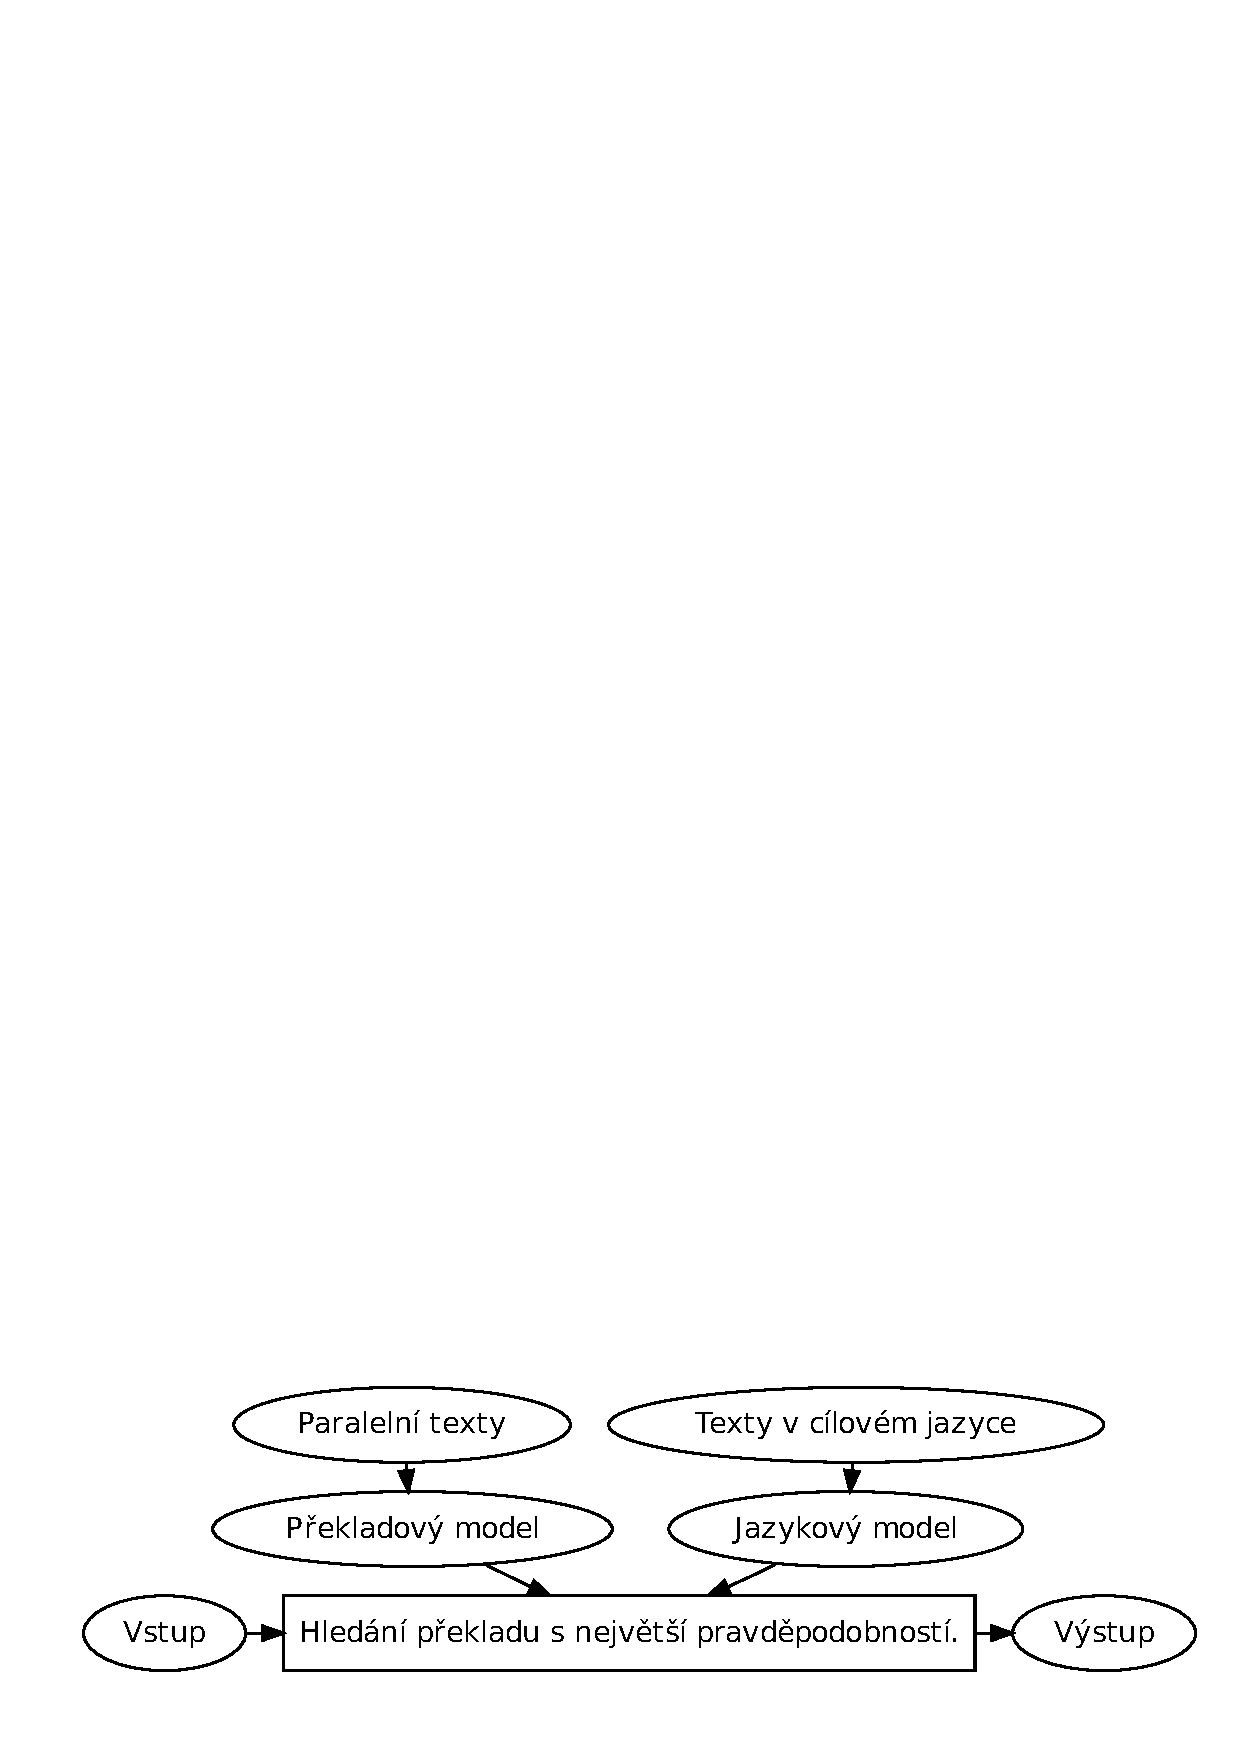
\includegraphics[width=120mm]{pictures/phrase-based}}}
\caption{Architektura frázového překladového systému.}
\label{phrase-based}
\end{figure}

\begin{figure}[t]
\centerline{\mbox{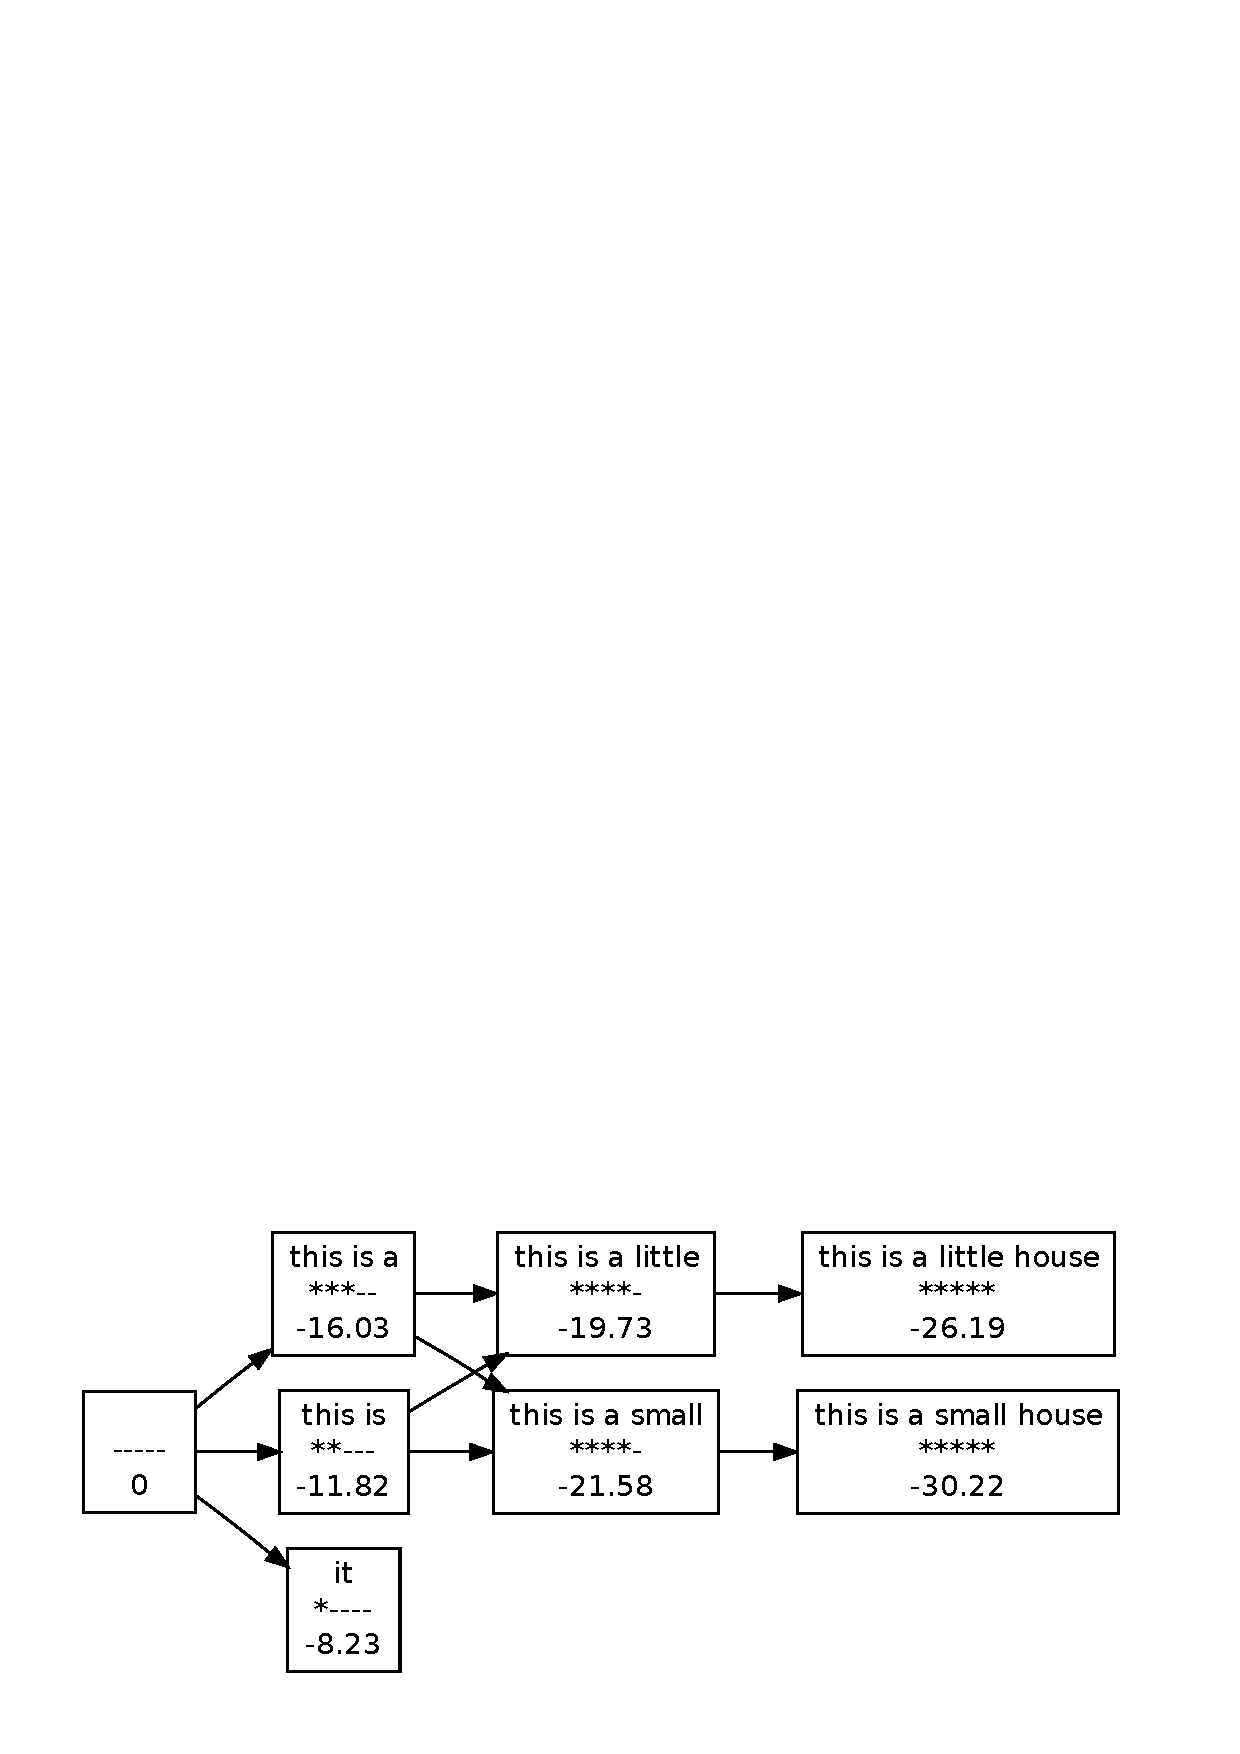
\includegraphics[width=120mm]{pictures/lattice}}}
\caption{Graf slov, ve kterém frázový překladový systém hledá nejlepší překlad.}
\label{lattice}
\end{figure}

\begin{figure}[t]
\centerline{\mbox{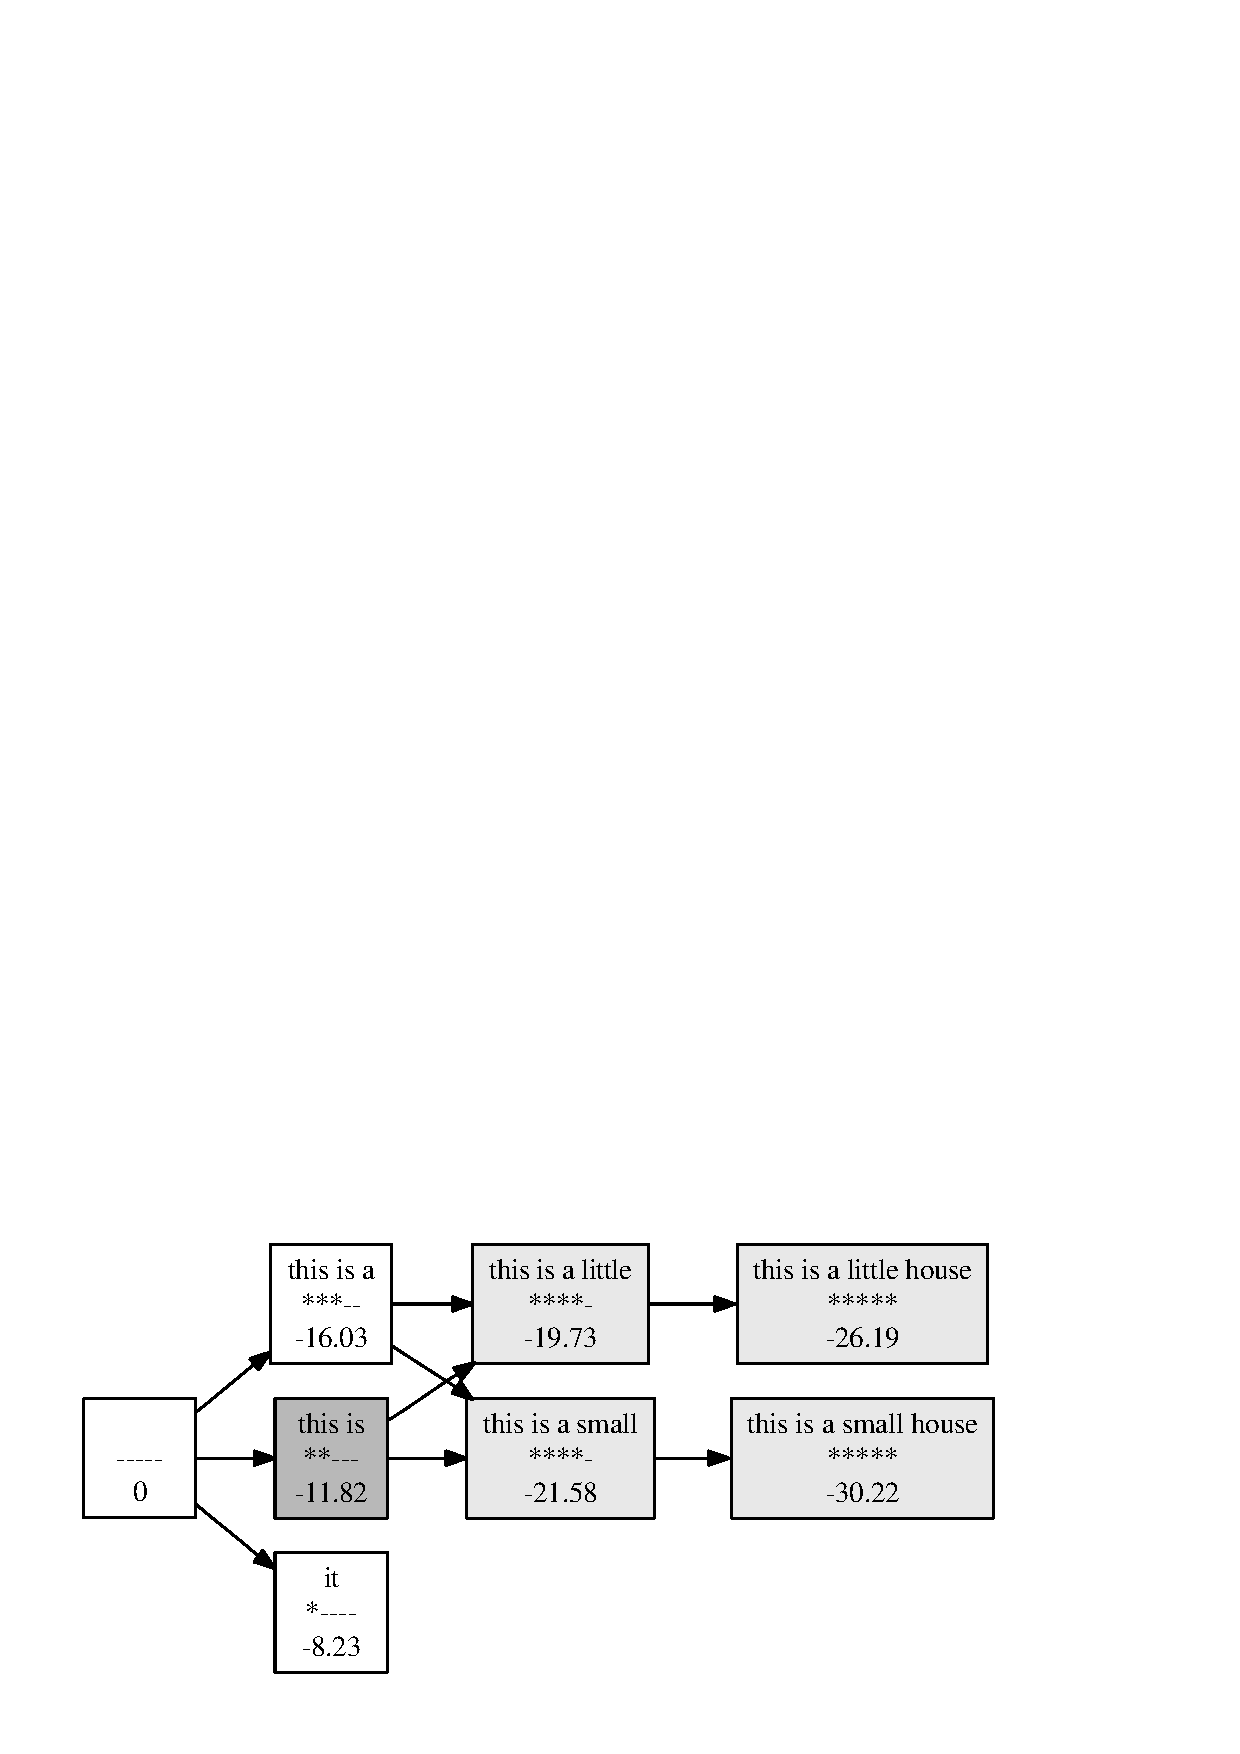
\includegraphics[width=120mm]{pictures/lattice-selected}}}
\caption{Frázový překladový systém rozšiřuje částečnou hypotézu.}
\label{lattice-selected}
\end{figure}

\begin{figure}[t]
\centerline{\mbox{\includegraphics[width=100mm]{pictures/non-zero-start}}}
\caption{Frázový překladový systém hledá hypotézu z neprázdné počáteční hypotézy.}
\label{non-zero-start}
\end{figure}

\section{Hledání nejlepších hypotéz}

Při generování překladu používá frázový systém strukturu, která se anglicky nazývá \clqq lattice\crqq , neboli graf slov. Graf odpovídá jednotlivým krokům překladového algoritmu frázových systému. Vrcholy jsou částečné hypotézy. Každá částečná hypotéza pokrývá nějakou část vstupu posloupností frází a má skóre určující relativní kvalitu překladu. Graf se skládá z orientovaných cest. Hrany znázorňují jednotlivé kroky algoritmu, který postupně rozšiřuje částečné hypotézy. Každá taková cesta začíná v takzvané nulové hypotéze, která reprezentuje stav, kdy nebylo ještě nic přeloženo. Cesta končí ve vrcholu pro který už frázový systém nedokáže rozšířit danou hypotézu. To se může stát buď proto, že mu překladový model nedává žádné možnosti pokračování, nebo je hypotéza konečná a všechna slova jsou již přeložena. Graf slov je podobný stromové struktuře, jenže o strom se nejedná protože se některé cesty mohou spojit. K tomuto spojení dvou cest dochází právě tehdy, když jsou dvě rozdílné částečné hypotézy rozšířeny frázovým systémem do jedné společné hypotézy.

Ukázka jednoho takového grafu slov je na Obrázku \ref{lattice}. Daný graf popisuje postup frázového systému při překladu věty \clqq das ist ein kleines haus\crqq  z němčiny do angličtiny. Pro názornost je tento graf velmi malý.

Obrázek \ref{lattice-selected} popisuje jeden krok překladového algoritmu. V tmavě označeném vrcholu se nachází částečná hypotéza, která pokrývá první dvě slova vstupní věty, tedy \clqq das ist\crqq  frází \clqq this is\crqq. Která slova jsou pokrytá znázorňuje vektor hvězdiček a podtržítek. Hvězdička na n-tém místě označuje že n-té slovo vstupní věty je již pokryto překladem. Algoritmus se pokusí tuto částečnou hypotézu rozvinout. Z překladového modelu získá dvě možnosti překladu fráze \clqq ein kleines\crqq  --- buď jako \clqq little house\crqq , nebo jako \clqq small house\crqq . Přidá tedy dva vrcholy a dvě hrany. V dalších krocích tyto hypotézy dále rozvíjí podobným způsobem až na konci získá dvě překladové hypotézy, které pokrývají všechna vstupní slova --- \clqq this is a little house\crqq  a \clqq this is a small house\crqq . Tyto hypotézy mají své skóre, takže je lze seřadit a jako výstup nabídnout hypotézu s nejvyšším skóre, což je hledaný nejlepší překlad. Frázové překladové systémy však umí poskytnout i takzvanou tabulku překladových možností Ta obsahuje i hypotézy s nižším skóre. To se hodí zejména proto, že metrika porovnávání dvou hypotéz není a nemůže být příliš exaktní. Překladatel často může použít pro překlad i hypotézu která nemá od překladového systému nejvyšší skóre.

Variant překladu může být obecně exponenciální množství. Graf slov se pak rozroste do obřích rozměrů a i pro malý překladový model a krátkou větu může obsahovat tisíce hran a vrcholů. Důležitým parametrem každého frázového překladového systému je tedy mimo kvality samotného překladu také rychlost získání překladu. Klíčový je v tomto ohledu rychlý algoritmus na procházení grafem slov. Moderní frázové systémy implementují algoritmus, který se snaží tento graf co nejvíce zmenšit. Algoritmus nerozvíjí hypotézy, které mají relativně nízké skóre a které tedy nemají šanci být rozvinuty do hypotézy použitelné na výstupu. Tento princip zahazování nepravděpodobných hypotéz výrazně zmenšuje exponenciální prostor hypotéz a umožňuje tím nalezení překladu v přijatelném čase.

%Obvyklým výstupem překladu je nejlepší plná hypotéza. Tedy hypotéza, která pokrývá všechny slova ve vstupní větě a zárověň má ze všech takových hypotéz nejvyšší skóre. Někdy se ovšem hodí získat i hypotézy s nižším skóre. Takovýto výstup se nazývá tabulka překladových možností, kde jednotlivé hypotézy tvoří řádky tabulky, které jsou seřazené podle skóre.

%Variant překladu může být obecně exponenciální množství. Pro rychlé hledání v těchto variantách implementuje Moses tzv. beam search algoritmus. Postup algoritmu při hledání zobrazuje Obrázek 2.2. Jedná se vlastně o orientovaný graf. Vrcholy grafu znázorňují částečné hypotézy. Každá taková částečná hypotéza pokrývá nějaká slova ze vstupu a má skóre, které určuje kvalitu hypotézy. Na začátku je překladu je prázdná hypotéza, která nepokrývá žádnou část vstupu. Na konci máme hypotézy které pokrývají celý vstup. Během překladu překladový systém postupně rozšiřuje exitující hypotézy o další fráze. Hypotéza s nejvyšším skóre je nabídnuta jako překlad na výstup. Pomocí tabulky překladovýchmožností dokáže Moses poskytnou i další hypotézy seřazené podle pravděpodobnosti.

%algoritmu známého pod názvem "beam search"

\chapter{Vývojová dokumentace}
Cílem této práce tedy bylo implementovat CAT systém, který by překladatelům umožňoval snadněji vytvářet kvalitní překlady. Pro podporu překladu měl systém používat frázový překladový systém. Implementovaný CAT systém je postaven na architektuře klient---server, což je výhodné zejména kvůli výpočetním a paměťovým nárokům které jsou pro použití frázového překladu s velkými překladovými a jazykovými modely nutné. Architektura klient---server umožňuje používání jedné instance překladového systému více klienty. Každý klient tak nemusí na svůj systém složitě instalovat celý překladový systém s těmito velkými jazykovými a překladovými modely.

\section{Překladový systém}

Jako frázový překladový systém byl zvolen Moses. Jedná se o open source frázový překladový systém s licencí GNU LGPL. Mezi jeho silné vlastnosti patří rychlý algoritmus pro průchod prostorem částečných hypotéz a také podpora pro různé výstupní formáty, včetně tabulky překladových možností, což jsou vlastnosti, které jsme pro náš projekt potřebovali. Při rozhodování bylo také důležité, že komunita kolem Mosese je poměrně velká a vývoj stále aktivní.

V implementovaném CAT systému jsme chtěli překladatelům nabízet dva druhy nápovědy. Prvním druh je tabulka překladových možností. Tuto nápovědu nabízí i caitra a Moses tento druh nápovědy nabízí jako jeden z druhů výstupu. Při implementaci bylo nutné tuto tabulku poskytnutou Mosesem upravit a odstranit z ní duplicity. Moses v tabulce překladových možností zobrazuje nejpravděpodobnější hypotézy překladu vstupní věty. Tyto hypotézy však mohou obsahovat stejné fráze pro překlad stejné části vstupní věty. V našem CAT systému tedy bylo nutné tyto duplicity odstranit, aby byla tabulka přehlednější a snadněji použitelná.

Dalším typem nápovědy jsou \clqq návrhy překladu\crqq . Jedná se o podobný druh nápovědy, jakou poskytují některé internetové vyhledávače. Během psaní textu do vyhledávacího políčka je uživateli navrhnuto několik variant pokračování zadaného textu a ten si pak jednu z takovýchto nápověd může vybrat pomocí kursorových šipek. Vyhledávací systém tyto nápovědy generuje pomocí statistiky nejčastěji zadaných vyhledávacích dotazů. Uživateli tedy dostane nejpravděpodobnější varianty pokračování při zadávání vyhledávacího dotazu. V našem CAT systému jsme chtěli, aby návrhy překladu fungovaly podobně a dávali překladateli nápovědu jak nejpravděpodobněji pokračovat z dané fázi překladu dále. Tyto návrhy překladu měly být získány z překladového systému.

Jednou z možností jak návrhy překladu získat by bylo využití tabulky překladových možností kterou generuje překladový systém. V této tabulce by se hledaly řádky se stejným prefixem jako má již přeložená část. Po odstranění prefixu v tomto řádku bychom získali návrhy překladu. Tento přístup má však dva problémy. Zaprvé může být celá tato tabulka dosti velká, během celého překladu věty by musela být v paměti a prohledávání v ní by bylo pomalé. Dalším problémem je, že se při překladu uživatel může dostane do fáze, která není zachycená nikde v grafu slov, tedy ani v tabulce překladových možností. I pro velké modely tato situace snadno nastane při použití cizího slova, které může být správným překladem, ale v překladovém modelu nemusí být nikde zachyceno. Tedy i kdyby byl částečný překlad věty správný, nemohl by náš CAT systém na základě výstupu z překladového systému nabídnout žádný návrh překladu.

Řešení těchto problémů je v intenzivnějším využívání překladového systému. Toho se nemusíme ptát jen na začátku překladu každé věty, ale můžeme se ho ptát v každé fázi překladu. K tomu je nutné překladový systém přizpůsobit tak, aby nám poskytoval překlady specifičtěji zadaných vstupů. Ve 2. kapitole je popsán způsob jakým frázový překladový systém běžně generuje překlady. Důležité je, že začíná z prázdné hypotézy, která nepokrývá žádná slova vstupní věty. V našem CAT systému by se hodilo, kdyby překladový systém uměl generovat i z počáteční neprázdné hypotézy, tak jak to zobrazuje \ref{non-zero-start}. Tato neprázdná hypotéza by reflektovala aktuální stav překladu. Musí tedy obsahovat informaci o textu již přeloženého textu, ale také vektor určující která slova vstupní věty jsou již přeložena. Tabulka překladových možností, která by vznikla z této neprázdné hypotézy by pak obsahovala hledané návrhy překladu.

Žádný z nám známých CAT systémů doposud nedisponuje podobnou funkcionalitou jakou jsou překladové návrhy. Její implementace byla jedním ze základních cílů tohoto projektu. Moses však generovat překlad z neprázdné hypotézy neuměl. Nejdříve tedy bylo nutné implementovat rozšíření Mosese, díky kterému by tento překladový systém dokázal na vstupu kromě zdrojového textu přijímat i informace o již přeložených částech vstupu a textu překladu. Informace o již přeložených částech je vektor, který určuje pro každé slovo, jestli se má překládat, nebo je již přeložené. Bez použití vektoru by se tento vstup dal simulovat tak, že by se ze vstupního řetězce pouze odstranila určitá slova. Pro překladový systém je důležité znát i text dosud přeložené části. Jazykový model překladového systému totiž porovnává sousední slova a pravděpodobnost sousedního výskytu slov se pak promítá do výsledného skóre překladové hypotézy. Text již přeložené části je tedy důležitý pro plynulejší navázání poskytovaných návrhů překladu.

Rozšířili jsme tedy Mosese tak, aby přijímal speciální druh vstupu s těmito informacemi navíc. Tento vstupu začne Moses přijímat při spuštěném přepínači {\tt -continue-partial-translation}\footnote{http://www.statmt.org/moses/?n=Moses.AdvancedFeatures\#ntoc25}, nebo zkráceně {\tt -cpt}. Příklad jednoho takového požadavku na Mosese může vypadat takto:\\

{\tt echo "that house ||| 10001 ||| das ist ein kleines haus" \textbackslash \\ | moses -f moses.ini -continue-partial-translation } \\

Program moses získá na vstupu řetězec, který je pomocí sekvence \clqq {\tt |||}\crqq  rozdělen na tři části. První část je řetězec s textem hotového překladu. Druhou částí je vektor nul a jedniček, kde symbol \clqq 1\crqq  na místě n říká, že nté slovo vstupní věty bylo již přeloženo a symbol \clqq 0\crqq  říká, že ještě přeloženo nebylo. Poslední částí je samotná věta na překlad. Pokud na vstupu není řetězec, který by odpovídal tomuto formátu, intepretuje Moses tento vstup, přestože má zapnutý přepínač {\tt -continue-partial-translation} jako normální vstupní větu.

\section{Server}

Pro implementovaný CAT systém bylo dále potřeba vytvořit server, který by přijímal požadavky od klienta, následně je předal Mosesovi. Ten by je zpracoval a vrátil zpět. Server by tento výstup zpracoval a vrátil klientovi. Moses dokáže generovat různé druhy výstupů. Pro naše účely se nejlépe hodila tabulka překladových možností. Jeden řádek takového výstupu má tvar řetězce: \\

{\tt 84 ||| it is small  ||| d: 0 lm: -20.8498 w: -3 tm: -3.21888 \\ ||| -24.0687 ||| 0-1=0-1 2=2 } \\

Každý takový řádek odpovídá jedné hypotéze překladu. Pomocí sekvence \clqq {\tt |||}\crqq  je řádek rozdělen na pět částí. První částí je číslo požadavku. Moses postupně zpracovává věty k překladu ze vstupu a číslo požadavku je jediným způsobem jak rozlišit, kdy končí jedna jeho odpověď a začíná druhá. V druhé části je samotný text překladu této hypotézy. Třetí sloupec obsahuje informace o kvalitě překladu, z nichž se ve čtvrtém sloupci spočítá samotné skóre této hypotézy. Poslední sloupec obsahuje informace zarovnání, tedy která slova na vstupu jsou pokryta kterými frázemi na výstupu. V daném příkladě si můžeme představit, že se překládá věta \clqq das ist kleines\crqq  z němčiny do angličtiny a zarovnání nám říká, že hypotéza pokrývá slova \clqq das ist\crqq  frází \clqq it is\crqq  a slovo \clqq kleines\crqq  slovem \clqq small\crqq . Hypotézy jsou v tabulce řazeny od shora od nejvíce pravděpodobné hypotézy. Moses umožňuje omezit velikost vygenerované tabulky, tedy nastavit maximální množství řádků výstupu pro každý požadavek. Při vhodné velikosti tohoto omezení je tabulka dostatečně velká, tak aby obsahovala všechny použitelné nápovědy a zároveň není tak velká, aby nějak výrazně zvyšovala čas zpracování požadavku.

Prvním druhem požadavku klienta na server je tedy dotaz na tabulku překladových možností. Serveru v tomto případě stačí znát jediný parametr --- text vstupní věty. Tento text server předá Mosesovi, který začne generovat překlad z prázdné hypotézy a na výstup vrátí serveru řádky tabulky překladových možností. Server musí tento výstup zpracovat, každý řádek nejprve rozdělit podle zarovnání na jednotlivé fráze, podívat se jestli fráze není duplicitní a pokud je, tak ji z výsledku odstranit. Takto zpracovaný výstup z Mosese může vrátit klientovi.

Dalším druhem požadavku klienta na server je dotaz na návrh překladu. Server potřebuje od klienta kromě textu vstupní věty získat i již přeložený text a také vektor určující, která slova vstupního textu byla tímto překladem již pokryta. Tyto parametry předá Mosesovi ve formátu vstupu použitém při zapnutém přepínači {\tt -continue-partial-translation}. Moses opět vrátí tabulku překladových možností. Server v tabulce hledá návrhy překladu. Návrhy mají omezenou délku na maximální počet tří slov. Delší návrhy by byly pro překladatele nepřehledné a navíc by se mohlo stát, že by se jednotlivé návrhy lišily jen nepatrně, což by také vedlo k nepřehlednosti. Kromě délky je omezený i počet návrhů, tak aby se v nich ještě mohl překladatel orientovat. Při samotném generování návrhů z překladové tabulky si server vezme text překladu, zkrátí ho na maximálně tři slova, zkontroluje jestli už stejný návrh nevygeneroval, nebo jestli už nemá návrhů dostatek, a případně návrh použije. Jelikož je tabulka překladových možností seřazena podle skóre, jsou podle pravděpodobnosti seřazené i získané návrhy překladu.

Server komunikuje s klientem pomocí protokolu HTTP. Každý požadavek na server je standardním požadavkem HTTP typu GET s příslušnými parametry. Těžší byl výběr formátu pro pro výstupní data. Variant a standardů existuje nespočet. Mezi nejznámější patří standard XML. Ten je však kritizován pro svojí těžkopádnost, kvůli které je i reprezentace malých dat relativně velká. Byl proto zvolen formát JSON, což je formát používaný ve skriptovacím jazyce JavaScript. Vyniká nejen svou stručností a vyjadřovací jednoduchostí, ale také tím, že s ním nativně umí pracovat všechny moderní prohlížeče\footnote{http://caniuse.com/\#feat=json}.

Během vývoje serveru byla změněna celá platforma. Původně byl server vyvíjen celý v Javě. Implementovaný server má být vlastně jen tenkým a rychlým obalem nad překladovým systémem. A z tohoto důvodu byl nakonec server implementován v jazyce C/C++ který je pro účel implementace rychlého serveru vhodnější. Navíc v jazyce C existuje otevřená knihovna libmicrohttpd, která je vyvíjena jako součást projektu GNU. Tato knihovna umožňuje relativně snadno udělat z aplikace v C/C++ vícevláknový server HTTP. Jejím používáním tak odpadá nutnost složitého implementování tohoto protokolu.

Dalším požadavkem na server bylo, dokázal spolupracovat s více instancemi překladového systému. Implementovaný CAT systém podporuje více jazykových párů. Pokud překladatel překládá například z angličtiny do češtiny a chce pokračovat překladem jiného dokumentu z němčiny do češtiny, nemusí se klient připojovat k jinému serveru. Server tedy umí spustit více instancí překladového systému a pomocí parametru v požadavku HTTP dokáže rozlišit, kterou instanci překladového systému má pro získání dané nápovědy použít.

\section{Klient}
Klientská část CAT systému má sloužit k samotné interakci s překladatelem. Jako platforma byl zvolen web, respektive webová aplikace. Webové aplikace mají oproti těm desktopovým několik výhod. Jednou z těch největších je dostupnost na všech platformách. Se správným prohlížečem může uživatel webovou aplikaci používat na mnoha operačních systémech. Navíc má uživatel vždy k dispozici nejnovější verzi používané aplikace. Webové aplikace mají také mnoho negativ, která jsou však postupem času eliminována. Mezi jednu z největších překážek vývoje webových aplikací patřila dlouhou dobu nutnost pro každou akci uživatele načítat celou webovou stránku znova. Tento problém vyřešila rodina technologií známá pod označením AJAX \footnote{z anglického Asynchronous JavaScript and XML}. Kromě skriptovacího jazyka JavaScript využívá AJAX především rozhraní XMLHttpRequest, pomocí kterého dokáže prohlížeč načíst data ze serveru bez nutnosti překreslení celé stránky.

Na použití AJAXových požadavků stojí i implementace klientské části implementovaného CAT systému. Pomocí AJAXu jde v prohlížeči poskytovat překladovou nápovědu formou, která překladatele neobtěžuje. Problémem AJAXu je, že rozhraní XMLHttpRequest implementuje každý webový prohlížeč trochu jinak. Je tedy výhodné použít pro implementaci framework, který zavede nad tímto rozhraním určitou abstrakci. Programátor pak nemusí pro každý AJAXový požadavek řešit kompatibilitu v různých prohlížečích.

Klientská část měla být původně napsána pomocí frameworku Google Web Toolkit\footnote{http://code.google.com/intl/cs/webtoolkit/}, který umožňuje psát aplikaci v Javě a ta je následně převedena do JavaScriptové aplikace spustitelné ve webovém prohlížeči. Google Web Toolkit však alespoň ve verzi 1.7 ještě neměl všechny potřebné vlastnosti, zejména co se týče uživatelského rozhraní. Další vlastností frameworku, kterou jsme pro náš systém považovali za nevýhodu je silná návaznost na technologie společnosti Google a její platformu Google App Engine\footnote{http://jquery.com/}.

Klientská část byla tedy nakonec vyvinuta pomocí frameworku jQuery. Tento framework je vlastně JavaScriptová knihovna, která nejenže odstiňuje programátora od rozdílných implementací AJAXu v prohlížečích, ale obecně usnadňuje práci s JavaScriptem v prohlížeči. Hlavním úkolem klientské části je poskytovat překladateli nápovědy poskytované serverem tak, aby to co nejvíce zefektivnilo proces překladu. To s sebou obnáší i nutnost rozdělit zadaný text na menší části, typicky věty, které umožní při překladu pracovat v jednotlivých krocích. Dále je potřeba, aby byl implementovaný CAT systém schopen uložit překlad a nabídnout ho překladateli i při dalším otevření prohlížeče. Místo ukládání dokumentu na serveru bylo zvoleno lokální úložiště v prohlížeči pomocí metody Web Storage. Toto úložiště je implementováno ve většině moderních prohlížečů\footnote{http://caniuse.com/\#feat=namevalue-storage}.


\chapter{Implementace serverové části}

\section{Instalace}

\subsection{Běžná instalace}
Serverová část AJAX-CAT používá nástroje a knihovny, které jsou silně provázané s Linuxovým světem. Instalace na jiných platformách může být poměrně obtížná, ne-li nemožná. Tento instalační návod tedy předpokládá použití využití standardní Linuxové distribuce jako je například Ubuntu, nebo Debian. Také se předpokládá, že jsou dostupné všechny běžné Linuxové nástroje, jako je například BASH shell, nebo programy g++, či make.

Nejprve je potřeba nainstalovat překladový systém Moses. Na oficiálních stránkách Mosese je poměrně obsáhlý návod k zprovoznění
\footnote{http://www.statmt.org/moses\_steps.html}. S balíčkovacím systémem aptitude je jednodušší variantou instalovat Mosese pomocí debian balíku z repozitáře Ubuntu NLP\footnote{http://cl.naist.jp/$\sim$eric-n/ubuntu-nlp/}. Dále je potřeba získat nějaký překladový a jazykový model. Součástí instalačních instrukcí pro Mosese je i návod, jak vytvořit tyto modely. Další možností je si nějaké jednoduché hotové modely stáhnout\footnote{http://www.statmt.org/moses/?n=Moses.SampleData}. Pro spuštění CAT systému je potřeba mít pro Mosese vytvořený konfigurační soubor moses.ini, který obsahuje definice a parametry překladového a jazykového modelu.

Dále je potřeba nainstalovat knihovnu libmicrohttpd\footnote{http://www.gnu.org/software/libmicrohttpd/}. Nejprve je potřeba stáhnout svn repozitář: \\


{\tt svn checkout https://gnunet.org/svn/libmicrohttpd/ } \\


Instalovat samotnou knihovnu by pak mělo jít pomocí posloupnosti příkazů: \\


{\tt autoreconf -fi

./configure

make

make install} \\

Podrobné informace o instalaci knihovny libmicrohttpd jsou v textovém souboru INSTALL v jejím repozitáři.

Nyní by mělo být vše připraveno k sestavení samotného serveru. Z přiloženého CD stačí zkopírovat obsah adresáře ajax-cat-server na lokální disk. Před instalací je potřeba otevřít soubor Makefile a zadat do proměnné MICROHTTPD\_PATH cestu ke knihovně libmicrohttpd. Pokud byla tato knihovna nainstalována standardně, nemělo by být nutné nic měnit. Server se pak zkompiluje příkazem make. Po kompilaci by měl vzniknout spustitelný soubor ajax-cat-server. Ten si své parametry bere z konfiguračního souboru config.ini. Vzorem toho, jak by měl tento soubor vypadat je soubor server.ini.example. Ten se nachází v Příloze 1 této práce. Parametr [moses-path] určuje cestu k programu Moses. Parametr [translation-pair] definuje informace o každém překladovém páru. Na prvním řádku se uvádí název překladového páru, na dalším řádku je pak cesta ke konfiguračnímu souboru pro Mosese pro tento pár. Sekcí může být víc, server dokáže spustit pro více překladových párů více instancí Mosese. Dobrou konvencí je tyto soubory pojmenovávat podle normy ISO 639-1\footnote{http://www.loc.gov/standards/iso639-2/php/English\_list.php}. Například překladový pár pro překlad z češtiny do angličtiny by se měl jmenovat \clqq cs-en\crqq .

Po nastavení cest v konfiguračním souboru se již může spustit samotný server. Stačí spustit program ajax-cat-server. V terminálu by se měly objevit informace o startování serveru. Server je nastartován v okamžiku, kdy se pro všechny překladové páry \clqq x-y\crqq  v terminálu objeví zpráva \clqq Thread x-y ready\crqq . Potom lze serveru posílat HTTP GET zprávy na port 8888. Funkčnost serveru lze otestovat po otevření prohlížeče a zadání adresy: \\

{\tt http://localhost:8888/simple?pair=x-y\&q=kleines\%20haus} \\

Server by měl vrátit řetězec s překladem věty \clqq kleines haus\crqq  pomocí překladového páru \clqq x-y\crqq . Běh serveru se z terminálu ukončí stisknutím klávesy Enter.

\subsection{Virtuální systém}

Nejjednoduší variantou, jak na svém počítači zprovoznit server je pomocí virtuálního stroje. Tento virtuální stroj s operačním systémem Ubuntu 10.04 se nachází na přiloženém CD. Pro jeho spuštění je potřeba mít nainstalovaný program Virtualbox\footnote{http://www.virtualbox.org/}, který je dostupný pro platformy Linux, Windows, Mac OSX i další. Pro spuštění virtuálního systému s již nainstalovaným serverem je tedy nutné pomocí Virtualboxu spustit archiv ajax-cat.ova v adresáři virtualni\_stroj na přiloženém CD. Přihlašovací heslo do virtuálního systému je \clqq ajax-cat\crqq . Po přihlášení stačí v terminálu spustit soubor {\tt ajax-cat-server} v adresáři {\tt ~/ajax-cat-server}


\section{Implementační detaily}

Celá serverová část implementovaného CAT systému je vlastně tenkou vrstvou napsanou v jazyce C/C++ propojující překladový systém Moses s HTTP serverem postaveným nad knihovnou libmicrohttpd. Po spuštění začne server obsluhovat HTTP požadavky na portu číslo 8888. Tato část popisuje všechny druhy dotazů, které může server obdržet.


\subsection{Požadavek simple}
Pomocí požadavku simple lze získat jako odpověď nejlepší překlad věty v jednoduché textové formě. Požadavek má tvar: \\

{\tt http://localhost:8888/simple?pair=de-en\&q=das+ist } \\

Parametr {\tt pair } určuje jméno překladového páru, který má server použít. Parametr {\tt q } je zdrojový text zakódovaný do standardního kódování HTTP.

\subsection{Požadavek table}
Na požadavek table vrací překladovou tabulku pro zadaný text. Požadavek má tvar: \\

{\tt http://localhost:8888/table?pair=de-en\&q=das+ist } \\

Parametry mají stejný význam jako u předchozího požadavku. Server vrací překladovou tabulku ve formátu JSON. Část {\tt source } je polem slov ve zdrojovém textu. Část {\tt target } je pole řádků tabulky. Každý řádek obsahuje frázi. Každá fráze má kromě textu (parametr "t") také část určující kolik slov ve zdrojovém textu pokrývá (parametr "s"). Příklad odpovědi na výše uvedený požadavek: \\

{\tt \{"source":["das","ist"],
"target":[ 

[\{"t":"this is ","s":"2"\}],
 
[\{"t":"it is ","s":"2"\}],
 
[\{"t":"the ","s":"1"\},

\{"t":"is ","s":"1"\}]

]\} 

}

Překládá se tedy \clqq das ist\crqq  v překladovém páru \clqq de-en\crqq . Odpověď říká, že nejlepším nalezeným překladem je přeložení celého \clqq das ist\crqq  frází \clqq this is\crqq , druhou variantou je překlad \clqq it is\crqq  a v posledním řádku je nabídnut překlad slova \clqq das\crqq  jako \clqq the\crqq  a překlad slova \clqq ist\crqq  jako \crqq is\crqq .

\subsection{Požadavek suggestion}
Důležitým požadavkem je suggestion, ten jako odpověď posílá návrhy překladu. Kromě parametrů shodných s předchozími požadavky má navíc parametry {\tt translated} a {\tt covered}: \\

{\tt http://localhost:8888/suggestion?pair=de-en \\ \&translated=a+small\&covered=00110\&q=das+ist+ein+kleines+haus } \\

Parametr {\tt translated} je text již přeložené části. Parametr {\tt covered} je vektor jedniček a nul označující již přeložené části ve zdrojovém textu. Odpověď serveru je opět ve formátu JSON a v poli {\tt suggestions} vrací nejpravděpodobnější návrhy pokračování překladu. Návrhů je maximálně 5 a každý má délku maximálně 3 slova. Příklad odpovědi serveru na výše uvedený dotaz může být následující: \\

{\tt \{"suggestions":["is the house","the house is","is this house"]\} }

\subsection{Požadavek raw}
Požadavek raw vrací tabulku překladových možností tak, jak ji vrací serveru Moses. Tento dotaz je vhodný především pro ladící účely. Formát dotazu je podobný jako v předchozích případech: \\

{\tt http://localhost:8888/raw?pair=de-en\&q=das+ist } \\

\section{Přehled souborů}
Složka se serverovou částí obsahuje soubory Makefile, server.ini, server.ini.example a pokud je projekt zkompilovaný, tak i spustitelný soubor ajax-cat-server. Makefile je soubor s pokyny pro sestavovací program make. Soubor server.ini je inicializační soubor s informacemi o umístění Mosese a umístěním a jmény jednotlivých překladových párů. Ukázkou, jak by měl konfigurační soubor vypadat je soubor server.ini.example. Po prvním spuštění programu vznikne tmp, kde se nacházejí pojmenované roury, které slouží ke komunikaci s Mosesem. Kód serveru se nachází v souboru server.cpp ve složce src.

\section{Funkce a třídy}

\subsection{Funkce main}
Spouští celý server. Z inicializačního souboru zjistí, kde se nachází Moses a jaké překladové páry má spustit. Funkcí MHD\_start\_daemon spustí libmicrohttpd server na portu 8888 a řekne mu, aby požadavky zpracovával funkcí answer\_to\_connection. Dále spouští kontrolní vlákno s funkcí control\_thread, která jednou za čas kontroluje, jestli jsou všechny procesy s Mosesem stále aktivní.

\subsection{Funkce answer\_to\_connection}
Tato funkce je volána při každém dotazu na server. Načte všechny přípustné parametry, který dotaz může mít a rozhodne, který jazykový pár bude požadovat a jaký tvar odpovědi je žádán. V případě správného dotazu vrátí funkce kód 200 správné HTTP odpovědi a zařadí odpověď do fronty odpovědí. Tuto frontu obsluhuje knihovna libmicrohttpd, která data vrací správnému tazateli.

\subsection{Třída MosesPair}
Tato třída reprezentuje jeden jazykový pár. V konstruktoru dostane své jméno a cestu ke konfiguračnímu souboru pro Mosese. Tento konfigurační pár určuje jeden překladový pár. Dále konstruktor vytvoří pojmenovanou rouru, kterou bude získávat výstup z Mosese, a spustí Mosese s příslušným konfiguračním souborem: \\

{\tt moses -f moses.ini

-n-best-list - 100 distinct

-include-alignment-in-n-best true

-continue-partial-translation true

> tmp/en-de\_out.fifo 2>/dev/null } \\

Parametry říkají Mosesovi, aby na výstup vygeneroval tabulku překladových možností maximální velikosti 100 řádků. Konstruktor třídy pak svou instanci zařadí do mapy {\tt server}, kterou používá funkce answer\_to\_connection k rozlišení toho, který jazykový pár má použít k získání odpovědi. Pak se ještě sám zařadí do seznamu {\tt serversOrder}, který využívá následně spuštěné vlákno k určení, který jazykový pár ho spustil. Nakonec spustí nové vlákno ovládané statickou metodou {\tt reader}.

Součástí třídy je fronta požadavků typu Request. Instance třídy MosesPair přijímají požadavky od funkce answer\_to\_connection pomocí metody get\_translation. Ta vezme požadavek a zařadí ho do své fronty. Dále procesu s Mosesem pošle dva požadavky na překlad. Prvním požadavkem je skutečná věta, kterou chce přeložit, druhým následujícím požadavkem je \clqq nesmyslný řetězec\crqq . Díky tomuto \clqq nesmyslnému řetězci\crqq  může server z výstupu který mu poskytuje Moses poznat, kdy končí jedna a začíná další odpověď. Aby bylo přidání do fronty i předání dotazů z Mosese bezpečné (k jedné instanci Mosese se může snažit přistoupit v jeden okamžik více požadavků), je při těchto operacích prováděno zamykání mutexů queue\_mutex a moses\_mutex. Po předání dotazu do Mosese funkce požadavek zamkne a čeká, dokud nebude odemčen vláknem, které čte výstupy z Mosese.

Tímto vláknem je právě vlákno, které spouští konstruktor třídy MosesPair na konci svého běhu a reprezentuje ho metoda {\tt reader}. Tato metoda se připojí k pojmenované rouře do které posílá Moses svůj výstup a postupně ji čte. Moses do pojmenované roury posílá postupně tabulku překladových možností. Metoda přečte řádek z roury, ten nejprve pomocí třídy Line rozdělí na jednotlivé části a získá pořadové číslo požadavku. Z pořadového čísla na předchozím řádku tak dokáže rozlišit situaci, kdy Moses začíná vracet odpověď na další požadavek. Jelikož je do požadavků na Mosese vkládán i \clqq nesmyslný řetězec\crqq , jsou zajímavé pouze odpovědi se sudými čísly požadavku. Pro každou takovou odpověď vezme metoda požadavek z fronty a začne mu předávat ke zpracování jednotlivé řádky výstupu. Díky tomu, že Moses dává na výstup požadavky ve stejném pořadí v jakém je obdržel, jsou řádky vraceny správnému požadavku. Po předání posledního řádku výstupu z Mosese pak uvolní v požadavku zámek, což umožní, aby metoda get\_translation mohla vrátit odpověď na dotaz klientovi.

\subsection{Třída Request}
Od této třídy dědí všechny ostatní druhy požadavků na server. Semafor {\tt sem} se pomocí metody {\tt lock} zamyká na začátku zpracování požadavku a odemyká se pomocí metody {\tt unlock} na konci zpracování. Každý požadavek má dvě metody --- {\tt process\_line} a {\tt get\_result}.

Metoda {\tt process\_line} dostává postupně jednotlivé řádky tabulky překladových možností a podle druhu dotazu tento řádek zpracovává. Řádek tabulky překladových možností je reprezentován třídou {\tt Line}, která nabízí základní metody pro parsování každé překladové možnosti.

Metoda {\tt get\_result} je volána po přijetí posledního řádku z tabulky překladových možností a generuje text, který je vrácen klientovi jako odpověď na dotaz.

\subsection{Třída RawRequest}
Tato třída je potomkem třídy {\tt Request}. Odpovídá požadavku raw, tedy neprovádí žádné zpracování a metodou {\tt get\_result} vrací tabulku překladových možností ve stejném formátu jako Moses.

\subsection{Třída SimpleRequest}
Tato třída je potomkem třídy {\tt Request}. Odpovídá požadavku simple. Zpracovává pouze první řádek tabulky překladových možností ze které získá samotný text překladu.

\subsection{Třída TableRequest}
Tato třída je potomkem třídy {\tt Request}. Odpovídá požadavku table. Tento druh požadavku odstraňuje duplicitní fráze z tabulky překladových možností a po převedení do formátu JSON vrací tabulku klientovi.

Tabulka je reprezentována třídou {\tt Table}. Na začátku každého zpracování je vytvořena nová instance třídy {\tt Table}. Pokaždé když požadavek obdrží prostřednictvím metody {\tt process\_line} jeden řádek překladových možností, rozdělí ho na jednotlivé fráze reprezentované třídou {\tt Phrase}, které se pak snaží umístit do tabulky. Umístění se nepovede pokud v tabulce již v odpovídajících sloupcích stejná fráze byla, nebo pokud jsou odpovídající sloupce zaplněné jinými frázemi. Tabulka má totiž kvůli přehlednosti pouze omezené množství řádků. 

Na závěr zpracování požadavku je tabulka pomocí metody {\tt get\_result\_table} převedena do JSON formátu a vrácena klientovi.

\subsection{Třída SuggestionRequest}
Tato třída je potomkem třídy {\tt Request}. Odpovídá požadavku suggestion a poskytuje tedy návrhy překladu. Při zpracování řádku tabulky překladových možností získá pomocí statické metody {\tt get\_suffix} řetězec se třemi prvními slovy návrhu. Tento řetězec se poté snaží přidat do pole {\tt results} a kontroluje, zda v něm již stejná fráze není. Maximální počet návrhů je pro přehlednost omezen.

\subsection{Ostatní funkce a třídy}
Funkce {\tt explode} vezme řetězec a s použitím zadaného znaku jako oddělovače rozdělí řetězec na části, které pak vrátí v datovém typu {\tt vector}. Funkce {\tt jsonify} převádí řetězec pro použití dle standardu JSON. Funkce {\tt clear\_input} odstraňuje z řetězce znaky nových řádků. Tyto znaky totiž používá Moses k oddělení jednotlivých vstupů. Třída {\tt Logger} se používá k logování dotazů a jiných informací. Tento log vypisuje server na standardní výstup.

\chapter{Implementace klientské části}

Klientská část CAT systému je webová aplikace využívající moderní technologie jako AJAX či WebStorage.

\section{Instalace}
Pro spuštění aplikace je potřeba mít nainstalován moderní webový prohlížeč. Nejdůležitějším požadavkem na prohlížeč je, aby podporoval technologii lokálního úložiště Web Storage. Toto úložiště podporují všechny moderní browsery\footnote{http://caniuse.com/\#feat=namevalue-storage}. Dále je potřeba mít nainstalovaný webový server Apache s podporou pro PHP skripty.

Samotná instalace je pak snadná, stačí překopírovat složku ajax-cat-client do složky, kterou používá Apache pro spouštěné skripty. Na linuxových systémech je to typicky složka {\tt /var/www}.

Nyní stačí v prohlížeči zadat adresu {\tt http://localhost/ajax-cat/} a měla by se objevit úvodní stránka klientské části AJAX-CAT.

Potom je ještě pořeba propojit klientskou část se serverovou. Nejprve je potřeba upravit soubor {\tt libraries/pairs.js }. V něm je potřeba upravit pole {\tt pairs} tak, aby položky code odpovídali názvům překladových dvojic na serverové části. Položka description slouží jako název překladového páru prezentovaný uživateli. Pokud máme jen jeden překladový pár s kódem \clqq cs-en\crqq  a názvem \clqq czech-english\crqq , může vypadat definice proměnné {\tt pairs} takto: \\

{\tt var pairs =

[\{

"code":"cs-en",

"description":"czech-english"

\}]; } \\

Dále je potřeba dát klientské části HTTP adresu serverové části. Pokud server běží na localhostu a portu číslo 8888, není potřeba nic měnit. Jinak je potřeba upravit poslední řádky PHP skriptů {\tt proxy/suggestion.php} a {\tt proxy/table.php}.

Při použití virtuálního hosta není potřeba nic instalovat, stačí zadat výše uvedenou adresu do prohlížeče.

\section{Návod k použití}
Na titulní stránce se kromě záhlaví a zápatí objeví i sekce \clqq Your translations\crqq  a \clqq New translation\crqq . V sekci \clqq Your translations\crqq  se nachází seznam překládaných dokumentů, který je při prvním použití aplikace prázdný. Překlad nového dokumentu se zahájí vložením zdrojového textu do textové oblasti v sekci \clqq New Translation\crqq  a stisknutím tlačítka \clqq Start translating\crqq . Proběhne přesměrování na stránku {\tt document.html} s překládaným dokumentem. Každý dokument má svůj šestnáctimístný hash kód, který se nachází v hashové části URL dokumentu a slouží jako identifikátor dokumentu.

V záhlaví dokumentu se nachází jeho název a překladový pár který je použit k podpoře překladu. Název i překladový pár jdou změnit v nabídce po kliknutí na tlačítko \clqq Settings\crqq . Kliknutím na \clqq Save\crqq  se dokument uloží do lokální paměti prohlížeče. Kliknutím na \clqq Preview\crqq  se zobrazí dokument v textové formě vhodné pro jeho vyexportování.

Dokument je při začátku překladu rozdělen na věty. Věty zdrojového textu překladu se při zobrazení dokumentu nachází v levé části obrazovky. Jejich odpovídající překlady na straně pravé. Aktuálně překládaná věta se nachází v modrém boxu. Na jinou větu lze přepnou kliknutím myší na příslušnou větu, nebo pomocí kláves \clqq Page Up\crqq  respektive \clqq Page Down\crqq .

Aktuálně překládaná věta má v modrém boxu nejprve znění ve zdrojovém textu, pod ním je textová oblast do které překladatel píše překlad. Pod textovou oblastí se nachází seznam návrhů překladu vygenerovaný serverovou částí. Pro použití nápovědy může překladatel na návrh buď kliknout myší, nebo návrh vybrat pomocí kursorových šipek a stisknutí klávesy \clqq Enter\crqq . Stisknutím klávesy \clqq tabulátor\crqq  vybere překladatel jen první slovo návrhu.

Dalším druhem nápovědy je tabulka ve spodní části modrého boxu. Záhlaví tabulky tvoří slova aktuální zdrojové věty překladu. Kliknutím slovo v záhlaví zmodrá jeho pozadí. Slova s modrým pozadím určují části zdrojové věty které již překladatel přeložil. Této informace používá CAT systém v požadavku k serveru na vygenerování návrhů překladu.

Překladatel může kdykoliv přerušit překlad a později se k němu ve svém prohlížeči opět vrátit. Na úvodní stránce se mu v sekci \clqq Your translations\crqq  zobrazí všechny jeho překlady spolu s názvem překladového páru a procentem udávajícím, kolik vět je již přeloženo. Kliknutím myší se mu daný dokument znovu otevře. Po kliknutí na ikonku s křížkem má možnost daný dokument smazat z paměti prohlížeče.


% Ukázka použití některých konstrukcí LateXu (odkomentujte, chcete-li)
% \include{ukazka}

\include{zaver}

%%% Seznam použité literatury
%\include{literatura}

\openright

\def\bibname{Seznam použité literatury}
\bibliographystyle{czechiso}
\bibliography{prace}

%%% Tabulky v diplomové práci, existují-li.
%\chapwithtoc{Seznam tabulek}

%%% Použité zkratky v diplomové práci, existují-li, včetně jejich vysvětlení.
\chapwithtoc{Seznam použitých zkratek}

%%% Přílohy k diplomové práci, existují-li (různé dodatky jako výpisy programů,
%%% diagramy apod.). Každá příloha musí být alespoň jednou odkazována z vlastního
%%% textu práce. Přílohy se číslují.
\chapwithtoc{Přílohy}

\section{server.ini.example}
{\tt
~~~[moses-path]

path/to/moses \\

[translation-pair]

pair-name

path/to/moses.ini \\

[translation-pair]

another-pair-name

path/to/another/moses.ini
}

\end{document}

